\documentclass[conference]{IEEEtran}
\hyphenation{op-tical net-works semi-conduc-tor}

\let\labelindent\relax

\usepackage{float}
\usepackage{graphicx}
\usepackage{hyperref}
\usepackage{enumitem}
\usepackage{url}
\usepackage{outlines}
\usepackage{blindtext}
%\usepackage[backend=biber,style=authoryear]{biblatex}
%\addbibresource{bibliography.bib}

\begin{document}

\title{Statistical Analysis of Advanced Encryption Standard}
\author{\IEEEauthorblockN{David Josephs}
\IEEEauthorblockA{\small Southern Methodist University\\
Dallas, Texas\\
Email: josephsd@smu.edu}
\and
\IEEEauthorblockN{Hannah Kosinovsky}
\IEEEauthorblockA{\small Southern Methodist University\\
Dallas, Texas\\
Email: hkosinovsky@mail.smu.edu}
\and
\IEEEauthorblockN{Carson Drake}
\IEEEauthorblockA{\small Southern Methodist University\\
Dallas, Texas\\
Email: drakec@smu.edu}
\and
\IEEEauthorblockN{Volodymyr Orlov}
\IEEEauthorblockA{\small Southern Methodist University\\
Dallas, Texas\\
Email: vorlov@smu.edu}}

\maketitle

\begin{abstract}
Advanced Encryption Standard (AES) is one of the most common and widely used specification for the encryption of electronic data. AES is a block cipher with 128-bit internal state and 128/192/256-bit key (AES-128, AES-192, AES-256, respectively). No efficient attacks against AES are known up to date and the standard is considered practically secure. In this paper we perform an extensive statistical analysis of AES-128 output using NIST Statistical Test Suite and additional randomness tests with a goal to identify any bias in either the entirety of the encrypted output or in sequences of encryption blocks generated from input values created using a counter or a linear feedback shift register (LFSR). 
\end{abstract}

\IEEEpeerreviewmaketitle

\section{Introduction}

Advanced Encryption Standard is a symmetric key block cipher method established by the U.S. National Institute of Standards and Technology (NIST) in 2001. In AES the same key is used for both encrypting and decrypting the data. Since its introduction, AES has been adopted by the U.S. government and is now used for a variety of applications worldwide. There are three variants of AES: AES-128, AES-192 and AES-256, where the number after AES
indicates the key length used for encryption and decryption process. Since its adoption, the world has seen little progress in the cryptanalysis of this cipher.

One of the basic properties of AES is indistinguishability of its output from a random sequence of bits. An evaluation of the cipher's output using randomness tests is an important tool in cryptanalysis that helps to ensure the algorithm produces no distinguishable patterns which can be used to deduce an encryption key or a plain text input. For this reason, the evaluation of the output of the AES by means of statistical randomness tests is of great importance. This study analyzes randomness
of the output produced by the AES-128 block cipher using NIST statistical test suite and  the Diehard test battery.
\section{Statistical Randomness Tests}

Statistical tests for randomness take arbitrary length input sequence and analyze its distribution to determine if it is random, containing no recognizable patterns or regularities. Usually these tests produce a real number between 0 and 1, the p-value, which shows the probability of finding the observed, or more extreme, results with respect to certain randomness properties of the given input. There exists some Notable software implementations of these statistical tests for randomness, like
the NIST Statistical Test Suite or Diehard tests. Tests such as these can be used to evaluate the randomness of AES.

The NIST Test Suite consists of 15 tests specially designed to analyze
binary sequences:
\begin{itemize}
  \item Two frequency tests, for monobit and a block, that test the randomness of a sequence of zeroes and ones
  \item Two runs test: a simple test and a test for the longest run of ones in a block, which looks for uninterrupted sequence of identical bits in the tested message.
  \item Binary matrix rank test, which checks for linear dependencies among fixed-length substrings of the original sequence.
  \item Discrete Fourier transform test, which detects periodic  patterns that repeat and are near each other in the tested sequence.
  \item Overlapping and non-overlapping template matching tests, which detect generators that produce too many occurrences of a given non-periodic pattern.
  \item Maurer’s "Universal Statistical" test, which uses compression without loss to detect whether or not the compressed sequence has less information than the original message.
  \item Linear complexity test, which determines whether or not the sequence is complex enough to be considered random.
  \item Serial test,  which searches for number of occurrences of the $2^m$ m-bit overlapping patterns and makes sure that its frequency is approximately the same as would be expected for a uniformly distributed sequence.
   \item Approximate entropy test,  which compares the frequency of overlapping blocks of two consecutive lengths against the expected result for a random sequence.
   \item Cumulative sums test, that determines whether the cumulative sum of the partial sequences occurring in the tested sequence is too large or too small relative to the expected behavior of that cumulative sum for random sequences.
   \item Random excursions and random excursions variant tests, which determines if the number of visits to a particular state within a cycle deviates from what one would expect for a random sequence and detect deviations from the expected number of visits to various states in the random walk
  
\end{itemize}
 All NIST tests examine randomness for the whole binary sequence. In addition to that several tests are also able to detect local regularities. 

Aside from the NIST test suites, there are a few other test suites for testing the randomness of cryptographic pseudorandom numbers, such as the Dieharder test suit, SPRNG, and the test suite mentioned in  (Statistical Testing of Cryptographic Randomness, Demirhan et al., 2016), which combines the Knuth, Helsinki, Diehard, and SPRNG test batteries.

The reason for including these various tests is to cover a wider array of statistical methods in order to detect a lack of randomness in AES-128. The NIST test suite tests for various metrics such as entropy, frequency within a block, random excursions, etcetera. In contrast, the 26-test Dieharder battery tests for distributions, bit distances, overlapping permutations and sums, while the SPRNG battery (13 tests) covers more stochastic processes such as random walks and the Ising model (a
mathematical model of ferromagnetism), and the Helsinki test looks for correlations and blocks within the pseudorandom data. The Knuth battery contains a different set of tests, with sme overlap with the others, however still including some unique tests. 

\section{Experiments}

The system of experiments employed in this study consist of 4 blocks:

\begin{enumerate}
  \item A plaintext generator is first used to  generate the necessary datasets consisting of nine different categories of data
  \item AES-128 Cipher  is then used  to encrypt plaintext messages
  \item NIST tests suite are used to run basic tests against encrypted messages.
  \item Diehard/Dieharder tests suite then serves as a final, more stringent, level of tests. 
\end{enumerate}

All four components are schematically represented in \autoref{HighLevelSchema}. We will run all modules on the SMU ManeFrame II cluster to get as big of a chance to catch any non-random pattern in encypted messages as we can.

% capital h for HERE
\begin{figure}[H]
\centering
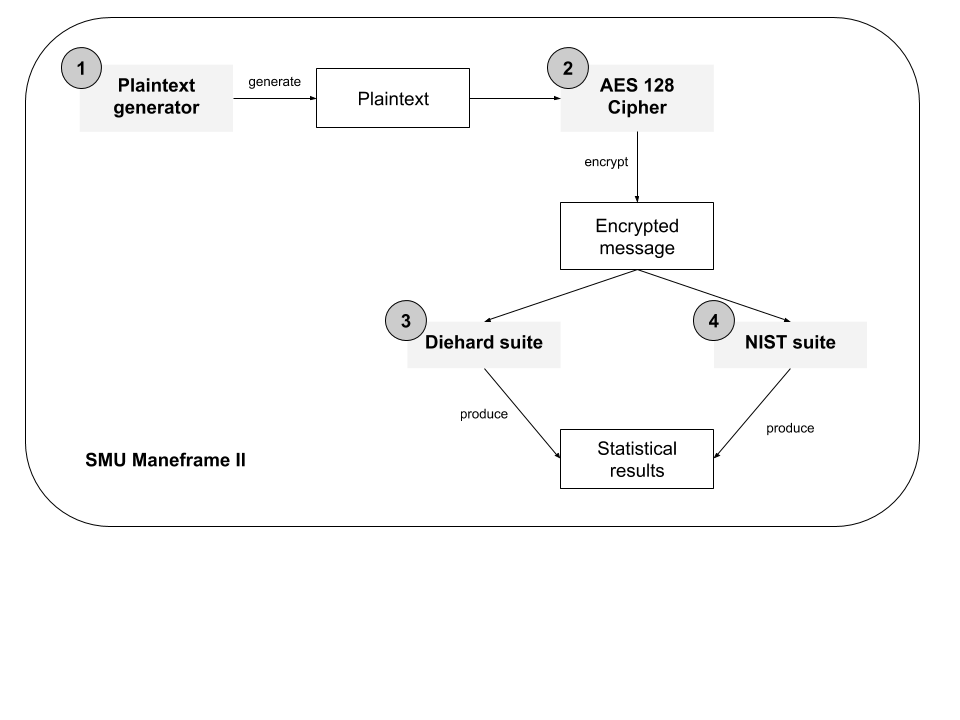
\includegraphics[width=3in]{imgs/HighLevelSchema.png}
\caption{Schematic layout of major components of the system}
\label{HighLevelSchema}
\end{figure}

%The nine categories of datasets have been selected because of their usefulness in evaluating the randomness of an algorithm's output. These nine categories are 128-bit key avalanche, Cipher Block Chaining Mode, Plaintext Avalanche, Low Density Plaintext, Low Density 128-Bit Keys, High Density Plaintext, High Density 128-Bit Keys, Plaintext/Ciphertext Correlation, and Random Plaintext/Random 128-Bit Keys.

\subsection{AES Datasets}
%The nine categories of datasets have been selected because of their usefulness in evaluating the randomness of an algorithm's output.
The following six categories of encrypted datasets have been selected because of their usefulness in evaluating the randomness of an algorithm's output.
\subsubsection{Low Density 128-Bit Key} 
 
The Low Density 128-Bit Key dataset consists of 300 sequences. Each sequence is made up of 8,257 ciphertext blocks. The ciphertext block is computed using a random plaintext block (unique to the individual sequence) and a low density 128-bit key. The first block utilizes a 128-key of all unset bits. Blocks 2-129 use a key consisting of 127 unset bits and one set bit, rotating the set bit across all 128-bit positions. For blocks 130-8,257, the key consists of 126 unset bits and two set bits, rotating the set bits in all unique combination across the 128-bit positions. All blocks are computed in ECB mode.

\subsubsection{Low Density Plaintext}

The Low Density Plaintext data set consists of 300 sequences. Each sequence is made up of 8,257 ciphertext blocks. The ciphertext block is computed using a random 128-bit key (unique to the individual sequence) and a low density plaintext block. The first plaintext block consists of 128 unset bits. Blocks 2-129 plaintext consisting of 127 unset bits and one set bit, rotating the set bit across all 128-bit positions. For blocks 130-8,257, the plaintext block consists of two set bits and 126 unset bits, rotating the set bits in all unique combination across the 128-bit positions. All blocks are computed in ECB mode.

\subsubsection{High Density 128-Bit Key}

The High Density 128-Bit Key dataset consists of 300 sequences. Each sequence is made up of 8,257 ciphertext blocks. The ciphertext block is computed using a random plaintext block (unique to the individual sequence) and a high density 128-bit key. The first block utilizes a 128-key of all set bits. Blocks 2-129 use a key consisting of 127 set bits and one unset bit, rotating the unset bit across all 128-bit 	positions. For blocks 130-8,257, the key consists of 126 set bits and two unset bits, rotating the set bits in all unique combination across the 128-bit positions. All blocks are computed in ECB mode.

\subsubsection{High Density Plaintext}
The High Density Plaintext dataset consists of 300 sequences. Each sequence is made up of 8,257 ciphertext blocks. The ciphertext block is computed using a random 128-bit key (unique to the individual sequence) and a high density plaintext block. The first plaintext block consists of 128 set bits. Blocks 2-129 plaintext consisting of all set bits and one unset bit, rotating the unset bit across all 128-bit positions. For blocks 130-8,257, the plaintext block consists of two unset bits and 126 set bits, rotating the unset bits in all unique combination across the 128-bit positions. All blocks are computed in ECB mode.

\subsubsection{Random Plaintext/Random 128-Bit Key} \label{sssec:RPK}
The Random Plaintext dataset consists of 300 sequences. Each sequence is made of 8,257 ciphertext blocks. To make each sequence, a random 128-bit key is first produced. Then that key is concatenated with 8,257 random plaintext blocks in ECB mode to generate the ciphertext sequence. 
\subsubsection{Plaintext/Ciphertext Correlation}
The Plaintext/Ciphertext Correlation is generated in order to study how plaintext-ciphertext pairs relate. 300 sequences were again generated, with a block length of 8,257, following the methods seen in \autoref{sssec:RPK}. The original plaintext is then XOR'd with the produced ciphertext, producing the dataset for analysis.
	
\subsection{Analysis}

All tests are implemented Python and C programming languages. For NIST test suite, we use modified Ilja Gerhardt's implementation \footnote{NIST implementation starter kit https://bit.ly/2Gkjdu1}. For Diehard test suite, we use Robert G. Brown’s Dieharder implementation of this suite. \footnote{Dieharder implementation https://bit.ly/2Sm325J}. Both implementations require some additional work from our side to run on SMU ManeFrame II cluster. 

%\cite{testsuite2}
%bibtex is not working on this cite but we can fix that later!

%\printbibliography 

\end{document}
